% Homework template created by Jonathan Wheeler
% for use at Stanford University.
% Edited by Lucas Saldyt
%
% Adapted from a jhwhw.cls file I found on
% github.
%
% In sublime, use Cmd-L, backspace to 
% clear auxiliary files 
% Better yet, don't use sublime.

% \usepackage{amsthm}

\documentclass[notitlepage]{homework}

\usepackage{amssymb}
\usepackage{amsmath}
\usepackage[parfill]{parskip}
\usepackage{minted}
\usepackage{graphicx}
\usepackage{tikz}
\usepackage{pgfplots}
\usepackage[euler]{textgreek}
\usepackage{multicol}
\usepackage{siunitx}
\usepackage{subcaption}

\pgfplotsset{compat=1.13}
\usetikzlibrary{decorations.pathmorphing,shapes}
\usepgfplotslibrary{fillbetween}
\usetikzlibrary{calc}

\newcommand{\AssignmentName}{MAT 300 3-26 HW}

\author{Lucas Saldyt}
\title{\AssignmentName}


\begin{document}
% Used in syntax highlighting
\definecolor{bg}{rgb}{0.95,0.95,0.95}

\begin{titlepage}
	\begin{center}
		{\Large \AssignmentName}
		
		\bigskip

		\begin{tabular}{rl}
			ID: & 1213399809 \\ % TODO
            Name: & Lucas Saldyt (lsaldyt@asu.edu) \\ % TODO
			Collaborators: & $\varnothing$
		\end{tabular}

		\bigskip

	\end{center}

	\toccontents

	\vfill

\end{titlepage}

\problem{5.2.10}

\begin{theorem}
Suppose that $h \colon A \to B$ and $k \colon B \to C$ are functions. If $h$ and $k$ are both one-to-one and onto, $(k \circ h)^{-1}$ is a function and $(k \circ h)^{-1} = h^{-1} \circ k^{-1}$.
\end{theorem}

\solution

\part 
\begin{proof}
First, since $h$ and $k$ are both one-to-one and onto, then $k \circ h$ is also one-to-one and onto, by a previously proven theorem.
Similarly, if any function $f$ is one-to-one and onto, then $f^{-1}$ is also a function, which is one-to-one and onto.
Thus, $(k \circ h)^{-1}$ is a function, which is one-to-one and onto.
Now, $k \circ h$ will map $A$ to $C$. $h^{-1}$ maps $B \to A$ and $k^{-1}$ maps $C \to B$. Thus, $k^{-1} \circ h^{-1}$ maps $C \to A$, as does $(k \circ h)^{-1}$.
Also, both $(k \circ h)^{-1}$ and $h^{-1} \circ k^{-1}$ are equal to $h^{-1}(k^{-1}(x))$ (The first instance is such because it is the inverse of $k(h(x))$, the second case is just a re-writing). Thus, they are equal.
\end{proof}

\problem{5.3.12}

Let $f \colon A \to B$ be a function.
\begin{enumerate}
    \item Give an example of a function $f \colon A \to B$ and two subsets $X$ and $Y$ of $A$ such that $f(X\cap Y) \neq f(X)\cap f(Y)$
    \item Show that $f(\cap_{\alpha \in \Lambda} T_\alpha) = \cap_{\alpha \in \Lambda} f(T_\alpha)$ for all choices of $f$ if and only if $f$ is one-to-one.
\end{enumerate}

\solution

\part 

Consider the sets $X = \{1\}, Y = \{2\}$, and $f = {(1, 1,), (2, 1)}$. Then, $f(X\cap Y) = \varnothing$, but $f(X) \cap f(Y) = \{1\}$.

\part

\begin{theorem}
Given a function $f$, the intersection of the images of all subsets of $A$ is equal to the image of the intersection of all subsets of $A$ if and only if $f$ is one-to-one.
\end{theorem}

\begin{proof}
Suppose the condition of the contrapositive, namely that $f$ is not one-to-one, i.e. that for some $b$ in the codomain, there are two distinct values $x$ and $y$ that map to another distinct value, $b$.
Now consider any subset $Y$, containing $y$ and any other subset $X$, containing $x$, where $y$ is not in $X$ and $x$ is not in $Y$. 
By definition, the intersection of $X$ and $Y$ will contain neither $x$ nor $y$.
However, since $x$ and $y$ both map to $b$, $b$ is an element of the intersection of the images on $X$ and $Y$.
Now recall that $b \neq x$ and $b \neq y$, so that the intersection of the images of $X$ and $Y$ is not equal to the image of the intersection of $X$ and $Y$.
Thus, by contrapositive, if $f$ is one-to-one, then the intersection of the images of all subsets of $f$ is equal to the image of the intersection of all subsets.

Now suppose the opposite direction, that the intersection of the images of $X$ and $Y$ is not equal to the image of the intersection of $X$ and $Y$. Call the intersection of images $C$ and the image of intersections $D$.
This means, by definition, that, without loss of generality between $C$ and $D$, there is some $c \in C$ and $c \not\in D$, and this $c$ is reachable by $f(x) | x \in A$.
However, the only way for $c$ to be in $C$ and not in $D$ is if $f$ is not one-to-one.
This is because either $c$ is in the intersection of the images or the image of the intersections, but not both.
This is possible in the case where $c$ is in the interesection of the images, but not the image of the intersections, when $x$ and $y$ map onto the same value, $b$, and thus $f$ is not one-to-one.
Thus, by contrapositive, if the intersection of the images of all subsets of $f$ is equal to the image of the intersection of all subsets, then $f$ is one-to-one.
\end{proof}

\problem{5.3.5}

Let $f \colon : \mathcal{R} \to \mathcal{R}$ be given by $f(x) = x^2$. Find the following:
\begin{enumerate}
    \item $f^{-1}(\{4\})$
    \item $f^{-1}([-2, 9])$
    \item $f^{-1}((1, 4])$
\end{enumerate}

\solution

\part 
$\{2\}$

\part
$[0, 3]$

\part
$[1, 2]$
  
\problem{5.5.13}

\solution

\part 

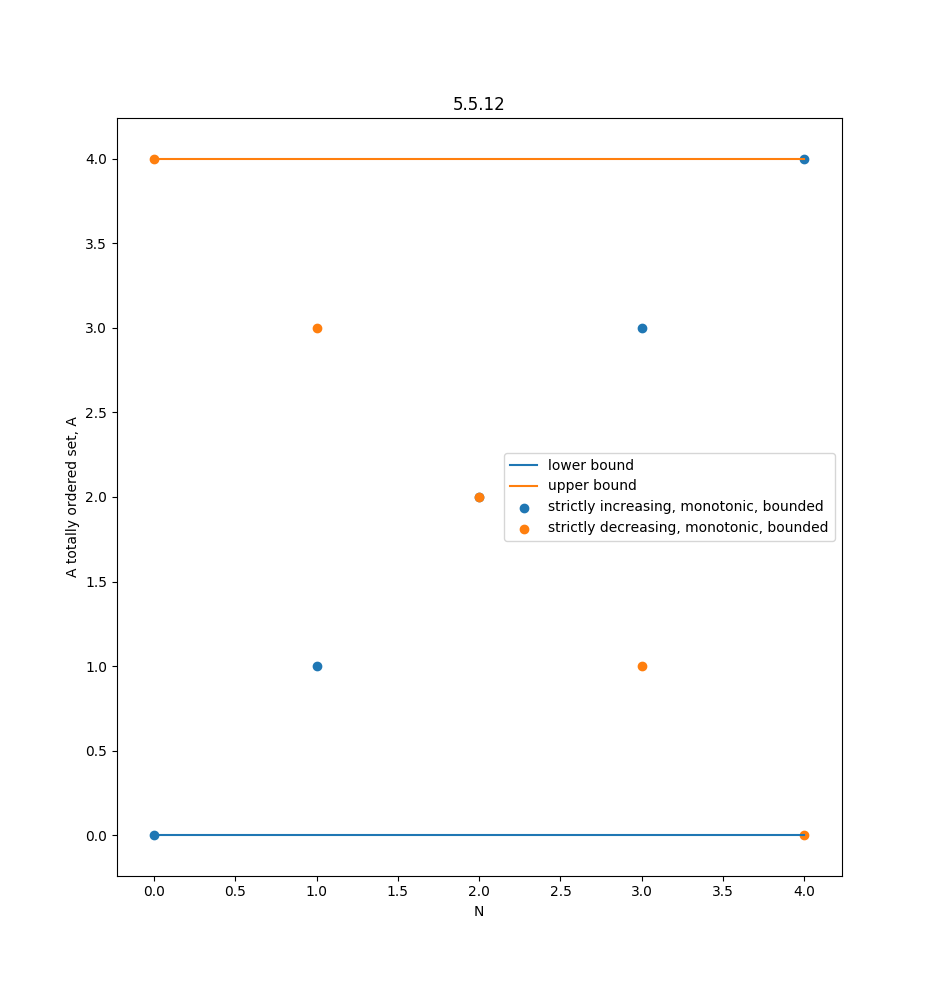
\includegraphics[scale=0.6]{0}


\problem{5.11}

Let $f \colon A \to B$ be a function. Let $X$ and $Y$ be subsets of $A$, and $U$ and $V$ be subsets of $B$.
\begin{enumerate}
\item Prove that $f^{-1}(U) \ f^{-1}(V) = f^{-1}(U \ V)$.
\item Prove that $f(X) \ f(Y) \subseteq f(X \ Y)$.
\end{enumerate}

\solution

\part 

\begin{theorem}
    The difference of the preimages of $U$ and $V$ is equal to the preimage of the difference of $U$ and $V$.
\end{theorem}
\begin{proof}
    The difference of the preimages contains all elements $x$ that reach $U$ but do not reach $V$. Similarly, the preimage of the difference of $U$ and $V$ contains all elements $x$ which reach $U$, but not $V$. Thus, these two sets are the same.
\end{proof}

\part

\begin{theorem}
    The difference of images on $X$ and $Y$ is a subset of the image on the difference of $X$ and $Y$.
\end{theorem}

\begin{proof}
    Consider the difference of images on $X$ and $Y$ (Call this $A$).
    This set consists of all elements reached by elements in $X$, but not reached by elements in $Y$.
    The image on the difference of $X$ and $Y$ ($B$) also consists of all elements which $X$ maps to, and so every element of $A$ is in $B$, i.e. $A \subseteq B$.
\end{proof}



\problem{5.12}

Let $f \colon A \to B$ be a function. Consider sets of the form $f(f^{-1}(S))$.

\begin{enumerate}
    \item Show that for all subsets $S$ of $B$, $f(f^{-1}(S)) \subseteq S$.
    \item Give an example to show that $f(f^{-1}(S))$ need not be equal to $S$.
    \item Complete and prove the following statement: $f(f^{-1}(S)) = S$ for all subsets $S$ of $B$ if and only if..
\end{enumerate}

\solution

\part 

$f$ maps $A \to B$, and $f^{-1}$ maps $B \to A$, then for some subset $S$ of $B$, $f^{-1}$ maps $S$ to $T \subseteq A$, and similarly $f$ maps $T \to V \subseteq B$.
However, $V$ is a subset of $S$, because $V$ consists of all elements which follow the form $f(f^{-1}(x))$, where $x$ is originally from $S$. $f(f^{-1}(x))$ cannot map onto an element not in $S$, because the "middle" set, i.e. $f^{-1}(S)$ is mapped to from $S$, and so the image of this set must be a subset of $S$.

\part

Consider $f(x) = x^2$ defined on the integers. Both $2$ and $-2$ map to $4$, but the inverse does not map back to $-2$.

\part

\ldots If and only if $f$ is one-to-one and onto.


\end{document}
